% 2015 全国Ⅱ理科 19(1) 解答图。斜投影按源卷第 966 页盒体前后方向：
% 前面为 y=0，后面为 y=10；EP 与 QF 按要求以虚线表示遮挡段。
% 方形边界 PQ、QF、FE、EP 是解答新增线，题面原盒体图不含这些线。
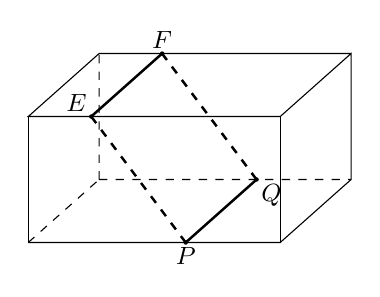
\begin{tikzpicture}[
  font=\small,
  x={(0.20cm,0cm)},
  y={(0.09cm,0.08cm)},
  z={(0cm,0.20cm)}
]
  % 长方体各顶点及题目所给截面点。
  \coordinate (A)  at (0,0,0);
  \coordinate (B)  at (16,0,0);
  \coordinate (C)  at (16,10,0);
  \coordinate (D)  at (0,10,0);
  \coordinate (A1) at (0,0,8);
  \coordinate (B1) at (16,0,8);
  \coordinate (C1) at (16,10,8);
  \coordinate (D1) at (0,10,8);
  \coordinate (E)  at (4,0,8);
  \coordinate (F)  at (4,10,8);
  \coordinate (P)  at (10,0,0);
  \coordinate (Q)  at (10,10,0);

  % 源盒体外轮廓；被前面遮挡的后底边与后左竖边用虚线。
  \draw (A)--(B)--(C)--(C1)--(B1)--(A1)--(D1)--(C1);
  \draw (A)--(A1) (B)--(B1);
  \draw[dashed] (A)--(D) (D)--(C) (D)--(D1);

  % 解答新增的正方形 E-P-Q-F；按给定要求虚线表示 EP、QF。
  \draw[dashed, line width=0.9pt] (E)--(P);
  \draw[line width=0.9pt] (P)--(Q);
  \draw[dashed, line width=0.9pt] (Q)--(F);
  \draw[line width=0.9pt] (F)--(E);

  \foreach \pt in {E,F,P,Q}
    \fill (\pt) circle (0.8pt);
  \node[above left, inner sep=1.5pt] at (E) {$E$};
  \node[above, inner sep=1.5pt] at (F) {$F$};
  \node[below, inner sep=1.5pt] at (P) {$P$};
  \node[below right, inner sep=1.5pt] at (Q) {$Q$};
\end{tikzpicture}
